%% In this subsection, along with an outline of the work that you plan to do -- from
%% the start to the end of your project -- you should also indicate what you think
%% could possibly change as you embark on and continually work on your thesis. In
%% the outline of your work, you might want to describe your methods of data
%% collection, any hardware or software you plan to build or implement, or any
%% algorithms you design. Who you are and what you bring to your work will also
%% help define what you plan to do. Here I quote Professor Neil Spring quite
%% broadly:
%% 
%%   Provide personal insight [to your thesis proposal]. You undoubtedly have a
%%   different way of viewing the world than anyone else, perhaps more theoretical
%%   or practical or empirical or operational. Maybe you think more like a user or
%%   more like a software engineer. [Maybe you had an interesting internship or
%%   spend a summer abroad.] Perhaps your undergraduate minor shapes your
%%   worldview.
%% 
%%   Wherever this project leads you, it's what you bring to the process that
%%   makes it interesting for everyone else. Focus on techniques. Focus on the
%%   methods and how they can be applied to solve a problem. You can make an
%%   exception if conflicating or changing results motivate further analysis.
%%   Often the inputs (workload, applications, processor speeds, network speeds)
%%   will change, and so the results (performace, comparisons) and conclusions
%%   will change with them.
%% 
%% You should also indicate what kind of equipment, facilities, data, or other
%% material you may need for the completion of your work. It is imperative that
%% you provide a timeline or a clear schedule that indicates a plan for your
%% thesis work. In this plan you and your thesis supervisor should come to an
%% agreement on goals for each month of the project including (but not limited to)
%% experiments, data collection, analysis, any refining, drafting of thesis, final
%% results, and revision of thesis. You are welcome to insert a chart with a
%% summary of your goals for each month. Most EECS Master's degree theses are
%% assigned a total number of 360 hours. We ask that you plan accordingly.

\section{Proposed Work}

  \begin{table}[h]
    \begin{tabularx}{\textwidth}{|c|X|}
      \hline
      \textbf{Month} & \textbf{Work to be completed} \\
      \hline
      December & Thesis proposal and ROS-based infrastructure for online particle filtering and associated visualization \\
      \hline
      January  & Experimentation with observational models for modeling neural detections. Writing submission to the RSS conference. \\
      \hline
      February & Refactoring code base and integration of the ROS particle filter and visualization components into Cora. \\
      \hline
      March    & Further integration/experimentation with the neural detector component (training on synthetic data, replacing with alternative architectures, training the neural component with error-correction on inference.) \\
      \hline
      April    & Development of thesis, documentation of work, and writing. \\
      \hline
      May      & Finalization of thesis and final documentation of work and code base. \\
      \hline
    \end{tabularx}
  \end{table}

  \begin{figure}
    \centering
    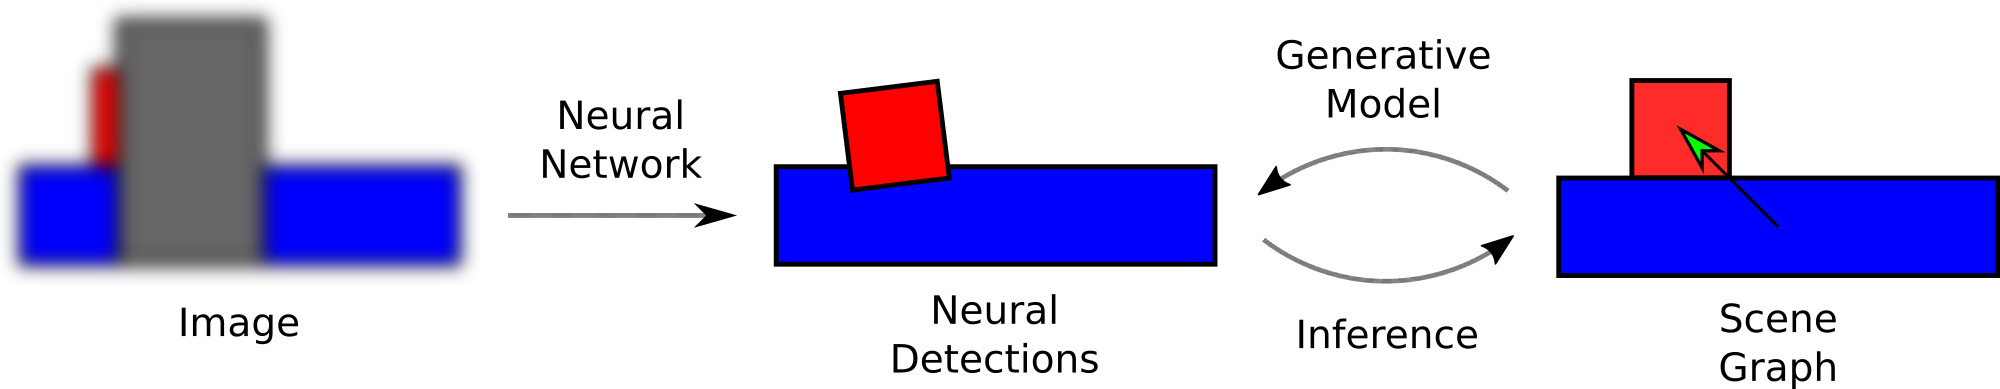
\includegraphics[width=\textwidth]{figures/neural-model.png}
    \caption{\small
      Neural detections can be inaccurate, and violate semantic relations
      between objects (eg. allow for object interpenetration). Given a neural
      detector, we can treat the flat and noisy detections as observations
      under a generative model, given prior structural information about the
      scene. Thus we implicitly model and correct for the failure modes of
      neural detections using uncertain prior structural knowledge. Using
      custom inference kernels, we can potentially recover the network's
      uncertainty, resolve impossible scenarios that violate prior knowledge,
      or even recover qualitative pose relationships like contact (green arrow)
      to enrich neural detections.
    }
    \label{fig:neural-model}
  \end{figure}
  

  \subsection{Neuro-predictive Generative Modeling}

    Modeling a rendering pipeline in a fully Bayesian way suffers from certain
    computational challenges. While guaranteed to converge to a correct
    posterior with unlimited compute time, the non-asymptotic properties of
    MCMC are poorly-understood. Preliminary work in inverse graphics techniques
    applied to structured scenes supports the hypothesis that naive
    analysis-by-synthesis approaches that leverage a full rendering pipeline
    often fail to explore all the modes of the posterior in reasonable time bounds
    \todo[WHO?]

    Concretely, for scene graph $\mathcal{S}$ and continuous parameterization
    $\vec{\nu}_\mathcal{S}$, a rendering-based likelihood relies on modeling
    the image data using a full rendering pipeline $R(\mathcal{S},
    \vec{\nu}_\mathcal{S}) = X$, where $X$ is a rendered image. For robustness,
    the likelihood is modeled not directly on $X$, but on a noisy function of
    the pixel data. The noise is modeled is a mixture of a uniform distribution
    on the range of possible values and a normal distribution with mean
    centered at the true rendered pixel value $R(\mathcal{S},
    \vec{\nu}_\mathcal{S})$ with fixed variance $\sigma^2$, leaving the full
    likelihood on noisy image data $Y$ as
    \begin{equation} \label{eq:1.1}
      p(Y | \mathcal{S}, \vec{\nu}_\mathcal{S}) = \prod_{r=1}^R\prod_{c=1}^C \paren{0.1 \cdot \frac{1}{D} + 0.9 \cdot \mathcal{N}(Y_{r,c}; R(\mathcal{S}, \vec{\nu}_\mathcal{S})_{r,c},\sigma)}
    \end{equation}

    \ref{eq:1.1} is very high-dimensional, making it prone to capture by local
    minima. Neural networks empirically demonstrate strong performance at
    locating strong \textit{maximum a posteriori} estimates in bounded compute
    time. Thus, we may consider combining neural techniques with MCMC to
    improve performance of inference.
    
    One perspective may consider neural networks as amortizations of the
    inverse generative procedure. Consider a neural detector $\phi_\mathcal{S}$
    that outputs poses under a given parametrization $\mathcal{S}$ (often a
    full unconstrained 6D pose), such that ideally $\phi_\mathcal{S}(R(\mathcal{S},
    \vec{\nu}_\mathcal{S})) = \vec{\nu}_\mathcal{S}$. Given image data $Y$, we
    can use the corresponding estimate $\phi_\mathcal{S}(Y)$ as an
    initialization for some MCMC technique.
    
    However, this method is rather unprincipled in that it uses a point
    estimate without uncertainty quantification, thus implicitly relying on
    $\phi_\mathcal{S}$ robustly predicting the mode of the distribution. This
    assumption is not guaranteed, and in fact when neural networks do fail,
    they often fail catastrophically, estimating wildly incorrect poses.
    Furthermore, because it is only a heuristic and not a full proposal
    distribution, it is not obvious how to combine neural detections across
    multiple timesteps into a coherent picture.  The issue fundamentally lies
    in the fact that this approach contains no way to reason about the behavior
    of the bottom-up proposals.  If we wish to robustly use these models, we
    need to leverage information about their behavior.

    Crucially, we can observe that the failure modes of these neural techniques
    are often quite predictable with the use of certain easy to compute
    statistics. When objects are too close or too far away, at strange angles,
    or heavily occluded, the neural detector is much more likely to fail. To
    account for these configurations, we propose instead modeling the neural
    detections as observations to a generative model that attempts to retrieve
    the latent scene graph $\mathcal{S}$ that predicts the detections from the
    neural network $\phi_\mathcal{S}(Y)$.

    A minimal observational model may be a simple mixture between a Gaussian
    and a uniform distribution over the entire space
    \begin{equation} \label{eq:1.2}
      p(\phi_\mathcal{S}(Y) | \mathcal{S}, \vec{\nu}_\mathcal{S}) = \mathcal{N}()
    \end{equation}

    Even such a simple observational model can be sufficient to filter some
    noise from the bottom-up proposal, by roughly modeling that the neural
    network sometimes makes mistakes (although in this case we don't use
    information about whether this is more or less likely at any given time).

  \subsection{Experimentation}

    The first task concrete task is creating the infrastructure sufficient for
    creating a minimal demo. For this we will develop an end-to-end system that
    uses DOPE+Gen+ROS to track a fixed set of objects, integrating prior
    knowledge about temporal consistency of object trajectories via state space
    modeling. For this, we can use a simple particle filter over object
    trajectories. This will help us nail down the end-to-end integration
    aspect, and also serves as the minimal example of ``filtering the output of
    a neural network via prior knowledge''. For simplicity we will initially
    work with an observation model of the form \ref{eq:1.2}. Even with this
    simple model, we hypothesis it is possible to filter spurious neural
    detections using physical assumptions of object persistence and intertial
    trajectories.

    Use the full pipeline to infer scene structure, integrating prior knowledge
    about scene graphs (e.g. contact relationships) as well as temporal
    consistency. This version will assume a static scene graph, but can later
    be adapted into an online algorithm by running the algorithm on the past
    e.g. 10 time steps of data in sliding windows.
    Use the full pipeline with a prior about temporal consistency of scene
    graphs (e.g. scene graphs change relatively infrequently).

    \subsubsection{Reversible Jump MCMC}

      Allowing MH moves between model parametrizations requires special
      mathematical consideration to ensure detailed balance is satisfied.
      \todo[Insert math]


  \subsection{Engineering Infrastructure}

    All of this experimentation requires sophisticated and novel infrastructure 
    for the prototyping of complex custom inference kernels and observational models
    to be applied in realtime 

    \subsubsection{Realtime Particle Filtering}


    \subsubsection{Visualization}

    \todo

    \subsubsection{Cora Project}

    \todo


  \subsection{Extensions}

    If time permits, there are several possible extensions to this work that
    may be considered. One relates \todo
